\section{Đặc tả chi tiết các use-case}

% ======================================================================================
% 4.1 QUẢN LÝ TÀI KHOẢN VÀ TRUY CẬP
% ======================================================================================
\subsection{Quản lý tài khoản và truy cập}

\subsubsection{Tổng quan}

\begin{figure}[H]
    \centering
    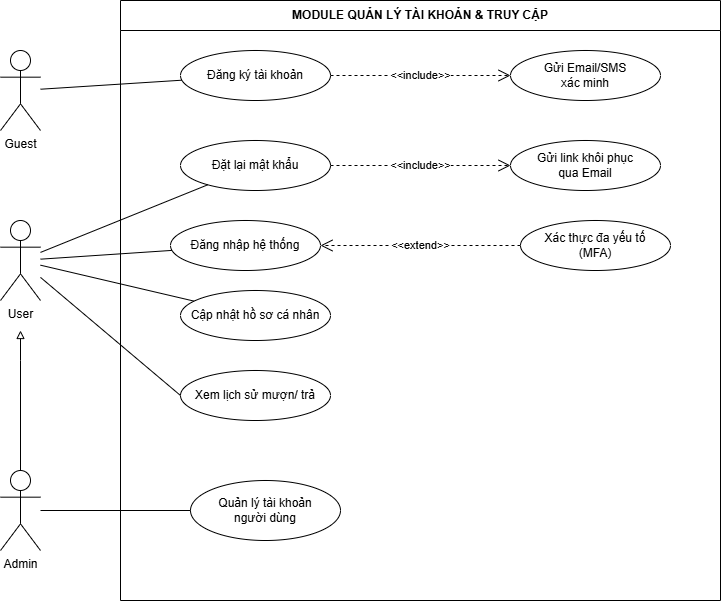
\includegraphics[width=0.8\linewidth]{Images/Quan_ly_tai_khoan_truy_cap.png}
    \vspace{10pt}
    \caption{Sơ đồ Use-case Quản lý tài khoản và truy cập}
    \label{fig:usecase_account}
\end{figure}

\subsubsection{Đặc tả chi tiết}

% --- UC: ĐĂNG KÝ TÀI KHOẢN ---
\begin{longtable}{|p{3.5cm}|p{11.5cm}|}
    \hline
    \textbf{Tên Use-case} & \textbf{Đăng ký tài khoản} \\
    \hline
    \textbf{Use-case ID} & UC-ACC-01 \\
    \hline
    \textbf{Tổng quan} & Cho phép người dùng chưa có tài khoản đăng ký trở thành thành viên của hệ thống. \\
    \hline
    \textbf{Actor} & Khách (Guest) \\
    \hline
    \textbf{Tiền điều kiện} & Khách truy cập vào trang đăng ký của hệ thống. \\
    \hline
    \textbf{Điều kiện kích hoạt} & Khách nhấn nút "Đăng ký". \\
    \hline
    \textbf{Các bước} & 
    1. Hệ thống hiển thị biểu mẫu đăng ký.\newline
    2. Khách nhập các thông tin bắt buộc (Họ tên, Email, Mật khẩu, v.v.).\newline
    3. Hệ thống kiểm tra tính hợp lệ của dữ liệu.\newline
    4. \textbf{[Include]} Hệ thống thực hiện luồng "Gửi Email/SMS xác minh" chứa mã OTP hoặc link kích hoạt đến thông tin liên lạc vừa đăng ký.\newline
    5. Khách nhập mã xác minh hoặc nhấp vào link.\newline
    6. Hệ thống xác thực mã, tạo tài khoản mới và lưu vào cơ sở dữ liệu.\newline
    7. Hệ thống hiển thị thông báo thành công. \\
    \hline
    \textbf{Hậu điều kiện} & Tài khoản được tạo thành công và trạng thái chuyển sang "Đã kích hoạt". \\
    \hline
    \textbf{Xử lý ngoại lệ} & 
    Ex1: Email/Số điện thoại đã tồn tại $\rightarrow$ Hệ thống báo lỗi và yêu cầu nhập lại.\newline
    Ex2: Nhập sai mã xác minh quá số lần quy định $\rightarrow$ Hủy phiên đăng ký. \\
    \hline
    \caption{Đặc tả Use-case Đăng ký tài khoản}
\end{longtable}

\newpage
% --- UC: ĐẶT LẠI MẬT KHẨU ---
\begin{longtable}{|p{3.5cm}|p{11.5cm}|}
    \hline
    \textbf{Tên Use-case} & \textbf{Đặt lại mật khẩu} \\
    \hline
    \textbf{Use-case ID} & UC-ACC-02 \\
    \hline
    \textbf{Tổng quan} & Hỗ trợ người dùng khôi phục quyền truy cập khi quên mật khẩu đăng nhập. \\
    \hline
    \textbf{Actor} & Người dùng (User - Tất cả vai trò) \\
    \hline
    \textbf{Tiền điều kiện} & Người dùng đã có tài khoản trên hệ thống nhưng không nhớ mật khẩu. \\
    \hline
    \textbf{Điều kiện kích hoạt} & Người dùng nhấn "Quên mật khẩu" tại màn hình đăng nhập. \\
    \hline
    \textbf{Các bước} & 
    1. Hệ thống yêu cầu người dùng nhập Email đã đăng ký.\newline
    2. Người dùng nhập Email và xác nhận.\newline
    3. Hệ thống kiểm tra sự tồn tại của Email trong cơ sở dữ liệu.\newline
    4. \textbf{[Include]} Hệ thống thực hiện luồng "Gửi link khôi phục qua Email".\newline
    5. Người dùng truy cập link khôi phục từ email của mình.\newline
    6. Hệ thống hiển thị màn hình đặt lại mật khẩu.\newline
    7. Người dùng nhập mật khẩu mới và xác nhận.\newline
    8. Hệ thống mã hóa và cập nhật mật khẩu mới, thông báo thành công. \\
    \hline
    \textbf{Hậu điều kiện} & Mật khẩu của người dùng được cập nhật mới. \\
    \hline
    \textbf{Xử lý ngoại lệ} & 
    Ex1: Email không tồn tại $\rightarrow$ Hiển thị thông báo "Không tìm thấy tài khoản với email này".\newline
    Ex2: Link khôi phục hết hạn $\rightarrow$ Yêu cầu người dùng thực hiện lại quy trình. \\
    \hline
    \caption{Đặc tả Use-case Đặt lại mật khẩu}
\end{longtable}

% --- UC: ĐĂNG NHẬP HỆ THỐNG ---
\begin{longtable}{|p{3.5cm}|p{11.5cm}|}
    \hline
    \textbf{Tên Use-case} & \textbf{Đăng nhập hệ thống} \\
    \hline
    \textbf{Use-case ID} & UC-ACC-03 \\
    \hline
    \textbf{Tổng quan} & Người dùng xác thực danh tính để vào hệ thống sử dụng các chức năng theo quyền hạn. \\
    \hline
    \textbf{Actor} & Người dùng (User - Tất cả vai trò) \\
    \hline
    \textbf{Tiền điều kiện} & Người dùng có tài khoản đang ở trạng thái hoạt động. \\
    \hline
    \textbf{Điều kiện kích hoạt} & Người dùng truy cập màn hình đăng nhập và điền thông tin. \\
    \hline
    \textbf{Các bước} & 
    1. Người dùng nhập thông tin danh tính (Email/Username) và Mật khẩu.\newline
    2. Hệ thống kiểm tra tính hợp lệ và đối chiếu dữ liệu.\newline
    3. \textbf{[Extend]} Nếu tài khoản được cấu hình bảo mật 2 lớp, hệ thống kích hoạt luồng "Xác thực đa yếu tố (MFA)", yêu cầu người dùng nhập mã OTP từ ứng dụng hoặc SMS.\newline
    4. Khởi tạo phiên làm việc (Session/Token) cho người dùng.\newline
    5. Chuyển hướng người dùng đến giao diện tương ứng với vai trò (Role). \\
    \hline
    \textbf{Hậu điều kiện} & Người dùng đăng nhập thành công, hệ thống ghi nhận lịch sử đăng nhập. \\
    \hline
    \textbf{Xử lý ngoại lệ} & 
    Ex1: Sai thông tin đăng nhập $\rightarrow$ Thông báo lỗi "Tài khoản hoặc mật khẩu không chính xác".\newline
    Ex2: Tài khoản đang bị khóa $\rightarrow$ Thông báo "Tài khoản của bạn đã bị khóa, vui lòng liên hệ Admin".\newline
    Ex3: Nhập sai mã MFA quá 3 lần $\rightarrow$ Tạm khóa đăng nhập trong 15 phút. \\
    \hline
    \caption{Đặc tả Use-case Đăng nhập hệ thống}
\end{longtable}

\newpage
% --- UC: CẬP NHẬT HỒ SƠ CÁ NHÂN ---
\begin{longtable}{|p{3.5cm}|p{11.5cm}|}
    \hline
    \textbf{Tên Use-case} & \textbf{Cập nhật hồ sơ cá nhân} \\
    \hline
    \textbf{Use-case ID} & UC-ACC-04 \\
    \hline
    \textbf{Tổng quan} & Người dùng tự thay đổi và cập nhật các thông tin cá nhân của mình trên hệ thống. \\
    \hline
    \textbf{Actor} & Người dùng (User) \\
    \hline
    \textbf{Tiền điều kiện} & Người dùng đã đăng nhập vào hệ thống. \\
    \hline
    \textbf{Điều kiện kích hoạt} & Người dùng truy cập vào phần "Hồ sơ cá nhân" và chọn "Cập nhật". \\
    \hline
    \textbf{Các bước} & 
    1. Hệ thống hiển thị form chứa thông tin cá nhân hiện tại.\newline
    2. Người dùng tiến hành chỉnh sửa các trường dữ liệu cho phép (Số điện thoại, địa chỉ, ảnh đại diện...).\newline
    3. Người dùng nhấn "Lưu".\newline
    4. Hệ thống kiểm tra ràng buộc dữ liệu.\newline
    5. Cập nhật dữ liệu vào cơ sở dữ liệu và hiển thị thông báo thành công. \\
    \hline
    \textbf{Hậu điều kiện} & Hồ sơ cá nhân của người dùng được cập nhật. \\
    \hline
    \textbf{Xử lý ngoại lệ} & 
    Ex1: Định dạng file ảnh đại diện không hợp lệ hoặc quá dung lượng $\rightarrow$ Cảnh báo lỗi và từ chối cập nhật file. \\
    \hline
    \caption{Đặc tả Use-case Cập nhật hồ sơ cá nhân}
\end{longtable}

% --- UC: XEM LỊCH SỬ MƯỢN/TRẢ ---
\begin{longtable}{|p{3.5cm}|p{11.5cm}|}
    \hline
    \textbf{Tên Use-case} & \textbf{Xem lịch sử mượn/ trả} \\
    \hline
    \textbf{Use-case ID} & UC-ACC-05 \\
    \hline
    \textbf{Tổng quan} & Cho phép người dùng tra cứu lại danh sách các tài liệu mình đã và đang mượn cùng trạng thái của chúng. \\
    \hline
    \textbf{Actor} & Người dùng (User) \\
    \hline
    \textbf{Tiền điều kiện} & Người dùng đã đăng nhập vào hệ thống. \\
    \hline
    \textbf{Điều kiện kích hoạt} & Người dùng chọn mục "Lịch sử mượn trả" trong bảng điều khiển cá nhân. \\
    \hline
    \textbf{Các bước} & 
    1. Hệ thống tiếp nhận yêu cầu từ người dùng.\newline
    2. Truy vấn cơ sở dữ liệu để lấy danh sách các giao dịch mượn/trả liên quan đến ID người dùng.\newline
    3. Hiển thị danh sách lên màn hình (bao gồm: Tên tài liệu, ngày mượn, ngày đến hạn, ngày trả thực tế, trạng thái, phí phạt nếu có).\newline
    4. Người dùng có thể sử dụng bộ lọc (theo thời gian, theo trạng thái) để tìm kiếm nhanh. \\
    \hline
    \textbf{Hậu điều kiện} & Không làm thay đổi trạng thái của hệ thống. \\
    \hline
    \textbf{Xử lý ngoại lệ} & 
    Ex1: Không có dữ liệu giao dịch $\rightarrow$ Hiển thị thông báo "Bạn chưa có lịch sử mượn tài liệu nào". \\
    \hline
    \caption{Đặc tả Use-case Xem lịch sử mượn/ trả}
\end{longtable}

\newpage
% --- UC: QUẢN LÝ TÀI KHOẢN NGƯỜI DÙNG (ADMIN) ---
\begin{longtable}{|p{3.5cm}|p{11.5cm}|}
    \hline
    \textbf{Tên Use-case} & \textbf{Quản lý tài khoản người dùng} \\
    \hline
    \textbf{Use-case ID} & UC-ACC-06 \\
    \hline
    \textbf{Tổng quan} & Cho phép người quản trị tìm kiếm, xem chi tiết, phân quyền, kích hoạt hoặc khóa tài khoản của người dùng. \\
    \hline
    \textbf{Actor} & Quản trị viên (Admin) \\
    \hline
    \textbf{Tiền điều kiện} & Quản trị viên đã đăng nhập và có quyền truy cập module quản trị hệ thống. \\
    \hline
    \textbf{Điều kiện kích hoạt} & Admin truy cập vào menu "Quản lý tài khoản". \\
    \hline
    \textbf{Các bước} & 
    1. Hệ thống hiển thị danh sách toàn bộ tài khoản người dùng.\newline
    2. Admin có thể thực hiện tìm kiếm hoặc lọc tài khoản theo vai trò, trạng thái.\newline
    3. Admin chọn một tài khoản cụ thể để thao tác (Khóa/Mở khóa tài khoản, Đặt lại mật khẩu, Thay đổi vai trò).\newline
    4. Admin xác nhận hành động thao tác.\newline
    5. Hệ thống ghi nhận thay đổi vào cơ sở dữ liệu, ghi log kiểm toán.\newline
    6. Hệ thống hiển thị thông báo thành công. \\
    \hline
    \textbf{Hậu điều kiện} & Trạng thái hoặc quyền hạn của tài khoản bị tác động được cập nhật. \\
    \hline
    \textbf{Xử lý ngoại lệ} & 
    Ex1: Admin cố gắng tự khóa tài khoản của chính mình $\rightarrow$ Hệ thống từ chối và cảnh báo lỗi vi phạm logic. \\
    \hline
    \caption{Đặc tả Use-case Quản lý tài khoản người dùng}
\end{longtable}

% ======================================================================================
% 4.2 QUẢN LÝ DANH MỤC VÀ BIÊN MỤC AI
% ======================================================================================
\subsection{Quản lý danh mục và Biên mục}

\subsubsection{Tổng quan}
\begin{figure}[H]
    \centering
    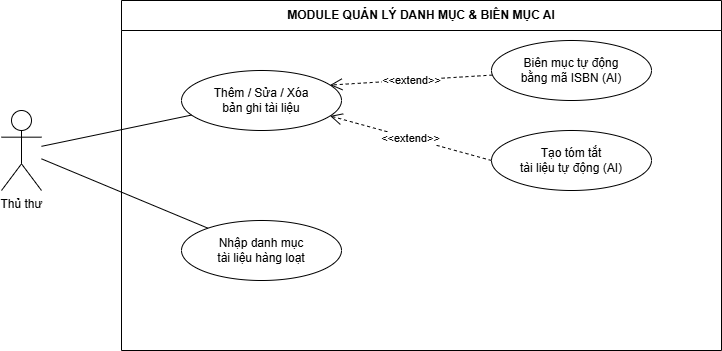
\includegraphics[width=0.8\linewidth]{Images/Quan_ly_danh_muc_bien_muc_AI.png}
    \vspace{10pt}
    \caption{Sơ đồ Use-case Quản lý danh mục \& Biên mục AI}
    \label{fig:usecase_catalog}
\end{figure}

\subsubsection{Đặc tả chi tiết}

% --- UC: THÊM / SỬA / XÓA BẢN GHI TÀI LIỆU ---
\begin{longtable}{|p{3.5cm}|p{11.5cm}|}
    \hline
    \textbf{Tên Use-case} & \textbf{Thêm / Sửa / Xóa bản ghi tài liệu} \\
    \hline
    \textbf{Use-case ID} & UC-CAT-01 \\
    \hline
    \textbf{Tổng quan} & Thủ thư thực hiện các thao tác quản trị tài liệu (CRUD) trong kho thư viện, bao gồm cập nhật thông tin sách, thêm mới hoặc xóa bỏ tài liệu hỏng/mất. \\
    \hline
    \textbf{Actor} & Thủ thư \\
    \hline
    \textbf{Tiền điều kiện} & Thủ thư đã đăng nhập vào hệ thống. \\
    \hline
    \textbf{Điều kiện kích hoạt} & Thủ thư truy cập vào trang "Quản lý danh mục tài liệu". \\
    \hline
    \textbf{Các bước} & 
    1. Hệ thống hiển thị danh sách tài liệu hiện có trong kho.\newline
    2. Thủ thư chọn một hành động: Thêm mới, Chỉnh sửa, hoặc Xóa.\newline
    3. Nếu Xóa: Thủ thư xác nhận xóa, hệ thống kiểm tra ràng buộc (sách có đang được mượn không) và thực hiện xóa mềm (Soft Delete).\newline
    4. Nếu Thêm/Sửa: Hệ thống hiển thị biểu mẫu thông tin tài liệu (Nhan đề, Tác giả, ISBN, Thể loại, Số lượng...).\newline
    \textit{** Điểm mở rộng (Extension Point):**}\newline
    - \textbf{[Extend]} Thủ thư có thể sử dụng chức năng \textit{"Biên mục tự động bằng mã ISBN"} (UC-CAT-03) để hệ thống tự điền form.\newline
    - \textbf{[Extend]} Thủ thư có thể sử dụng chức năng \textit{"Tạo tóm tắt tài liệu tự động"} (UC-CAT-04) nếu sách chưa có mô tả.\newline
    5. Thủ thư rà soát lại thông tin và nhấn "Lưu".\newline
    6. Hệ thống validate dữ liệu, lưu vào cơ sở dữ liệu và thông báo thành công. \\
    \hline
    \textbf{Hậu điều kiện} & Danh mục tài liệu được cập nhật thành công. \\
    \hline
    \textbf{Xử lý ngoại lệ} & 
    Ex1: Thiếu thông tin bắt buộc $\rightarrow$ Hệ thống bôi đỏ các trường thiếu và yêu cầu nhập đầy đủ.\newline
    Ex2: Mã tài liệu hoặc ISBN bị trùng lặp $\rightarrow$ Hiển thị thông báo "Mã ISBN đã tồn tại trong hệ thống". \\
    \hline
    \caption{Đặc tả Use-case Thêm / Sửa / Xóa bản ghi tài liệu}
\end{longtable}

\newpage
% --- UC: NHẬP DANH MỤC TÀI LIỆU HÀNG LOẠT ---
\begin{longtable}{|p{3.5cm}|p{11.5cm}|}
    \hline
    \textbf{Tên Use-case} & \textbf{Nhập danh mục tài liệu hàng loạt} \\
    \hline
    \textbf{Use-case ID} & UC-CAT-02 \\
    \hline
    \textbf{Tổng quan} & Cho phép Thủ thư import số lượng lớn tài liệu vào hệ thống cùng một lúc thông qua file chuẩn (CSV, Excel ). \\
    \hline
    \textbf{Actor} & Thủ thư \\
    \hline
    \textbf{Tiền điều kiện} & Thủ thư đã đăng nhập vào hệ thống. \\
    \hline
    \textbf{Điều kiện kích hoạt} & Thủ thư chọn chức năng "Nhập hàng loạt (Import)" tại giao diện quản lý danh mục. \\
    \hline
    \textbf{Các bước} & 
    1. Hệ thống hiển thị giao diện tải lên tệp tin và cung cấp file mẫu (Template).\newline
    2. Thủ thư tải lên tệp tin chứa dữ liệu danh mục.\newline
    3. Hệ thống đọc tệp, phân tích dữ liệu và hiển thị bản xem trước (Preview) các bản ghi hợp lệ và không hợp lệ.\newline
    4. Thủ thư xác nhận tiến hành Import.\newline
    5. Hệ thống ghi dữ liệu vào cơ sở dữ liệu và hiển thị báo cáo kết quả (Số dòng thành công, số dòng lỗi). \\
    \hline
    \textbf{Hậu điều kiện} & Nhiều bản ghi tài liệu mới được bổ sung vào hệ thống. \\
    \hline
    \textbf{Xử lý ngoại lệ} & 
    Ex1: Sai định dạng tệp (không phải CSV/Excel) $\rightarrow$ Hệ thống từ chối tệp và báo lỗi "Định dạng tệp không được hỗ trợ".\newline
    Ex2: Dữ liệu trong tệp chứa mã ISBN trùng lặp $\rightarrow$ Hệ thống bỏ qua dòng lỗi đó, ghi log báo cáo và import các dòng hợp lệ còn lại. \\
    \hline
    \caption{Đặc tả Use-case Nhập danh mục tài liệu hàng loạt}
\end{longtable}

% --- UC: BIÊN MỤC TỰ ĐỘNG BẰNG MÃ ISBN (AI) ---
\begin{longtable}{|p{3.5cm}|p{11.5cm}|}
    \hline
    \textbf{Tên Use-case} & \textbf{Biên mục tự động bằng mã ISBN } \\
    \hline
    \textbf{Use-case ID} & UC-CAT-03 \\
    \hline
    \textbf{Tổng quan} & Tính năng AI hỗ trợ tự động truy xuất và điền thông tin metadata của sách (Tên, Tác giả, Nhà XB, Thể loại) từ các nguồn dữ liệu bên ngoài thông qua mã ISBN. \\
    \hline
    \textbf{Actor} & Thủ thư \\
    \hline
    \textbf{Tiền điều kiện} & Đang ở luồng thực thi của Use-case "Thêm / Sửa / Xóa bản ghi tài liệu". \\
    \hline
    \textbf{Điều kiện kích hoạt} & Thủ thư nhập mã ISBN và nhấn nút "Lấy thông tin tự động". \\
    \hline
    \textbf{Các bước} & 
    1. Thủ thư nhập mã ISBN vào trường dữ liệu tương ứng.\newline
    2. Hệ thống gửi request chứa mã ISBN đến các API nguồn mở (Google Books, Open Library).\newline
    3. Hệ thống nhận chuỗi JSON trả về, dùng mô-đun phân tích để trích xuất các thực thể thông tin cần thiết.\newline
    4. Hệ thống tự động điền các thông tin trích xuất được vào các trường tương ứng trên biểu mẫu (Form).\newline
    5. Thủ thư kiểm tra, chỉnh sửa (nếu cần) và tiếp tục luồng của Use-case gốc. \\
    \hline
    \textbf{Hậu điều kiện} & Biểu mẫu nhập liệu được điền sẵn thông tin, tiết kiệm thời gian cho Thủ thư. \\
    \hline
    \textbf{Xử lý ngoại lệ} & 
    Ex1: Không tìm thấy sách với mã ISBN đã cung cấp $\rightarrow$ Hệ thống báo "Không tìm thấy dữ liệu tự động, vui lòng nhập thủ công".\newline
    Ex2: Lỗi kết nối API bên thứ 3 $\rightarrow$ Hệ thống báo lỗi timeout và yêu cầu thử lại sau. \\
    \hline
    \caption{Đặc tả Use-case Biên mục tự động bằng mã ISBN}
\end{longtable}

\newpage
% --- UC: TẠO TÓM TẮT TÀI LIỆU TỰ ĐỘNG (AI) ---
\begin{longtable}{|p{3.5cm}|p{11.5cm}|}
    \hline
    \textbf{Tên Use-case} & \textbf{Tạo tóm tắt tài liệu tự động} \\
    \hline
    \textbf{Use-case ID} & UC-CAT-04 \\
    \hline
    \textbf{Tổng quan} & Sử dụng mô hình ngôn ngữ lớn (LLM) để tự động sinh ra đoạn tóm tắt ngắn gọn (150-300 từ) cho các tài liệu chưa có phần mô tả. \\
    \hline
    \textbf{Actor} & Thủ thư \\
    \hline
    \textbf{Tiền điều kiện} & Đang ở luồng thực thi của Use-case "Thêm / Sửa / Xóa bản ghi tài liệu". Tài liệu đã có Nhan đề và Tác giả. \\
    \hline
    \textbf{Điều kiện kích hoạt} & Thủ thư nhấn nút "Tạo tóm tắt AI" tại trường Mô tả tài liệu. \\
    \hline
    \textbf{Các bước} & 
    1. Hệ thống thu thập các thông tin cơ bản hiện có trên form (Nhan đề, Tác giả, Thể loại).\newline
    2. Hệ thống đóng gói thông tin thành một Prompt và gửi đến AI Engine (VD: OpenAI/Gemini API).\newline
    3. AI Engine xử lý và trả về đoạn văn bản tóm tắt.\newline
    4. Hệ thống điền đoạn văn bản vào trường "Mô tả", tự động gắn nhãn "(Tóm tắt do AI tạo ra)".\newline
    5. Thủ thư đọc duyệt, chỉnh sửa hoặc yêu cầu AI tạo lại (Regenerate). \\
    \hline
    \textbf{Hậu điều kiện} & Sách có thêm phần tóm tắt nội dung hấp dẫn, hỗ trợ bạn đọc tìm kiếm dễ dàng hơn. \\
    \hline
    \textbf{Xử lý ngoại lệ} & 
    Ex1: Thông tin đầu vào quá ít (chỉ có nhan đề, không có tác giả) khiến AI không thể nhận diện đúng sách $\rightarrow$ AI trả về kết quả chung chung, Thủ thư từ chối kết quả và xóa bỏ. \\
    \hline
    \caption{Đặc tả Use-case Tạo tóm tắt tài liệu tự động}
\end{longtable}

% ======================================================================================
% 4.3 QUẢN LÝ LƯU THÔNG TÀI LIỆU
% ======================================================================================
\subsection{Quản lý lưu thông tài liệu}

\subsubsection{Tổng quan}
\begin{figure}[H]
    \centering
    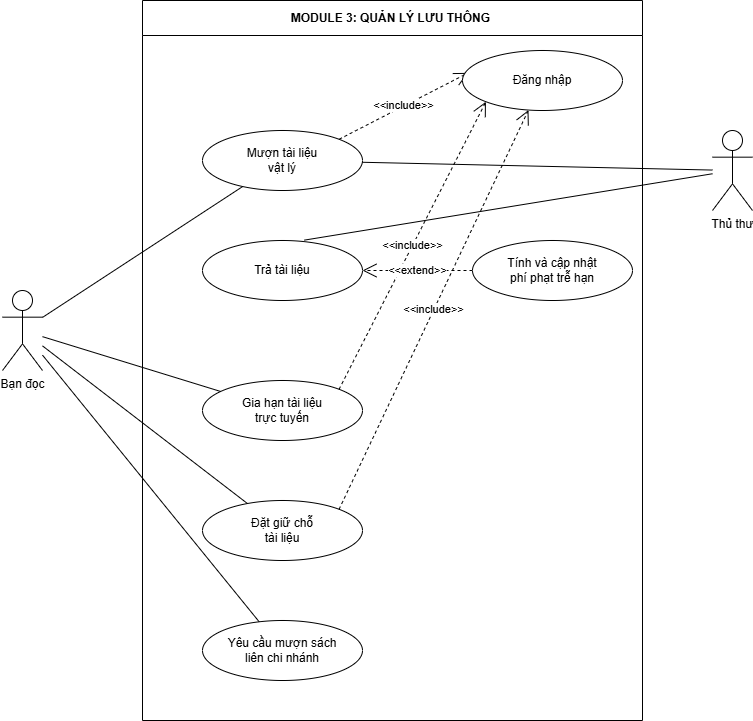
\includegraphics[width=0.8\linewidth]{Images/Quan_ly_luu_thong.png}
    \vspace{10pt}
    \caption{Sơ đồ Use-case Quản lý lưu thông tài liệu}
    \label{fig:usecase_circulation}
\end{figure}

\subsubsection{Đặc tả chi tiết}

% --- UC: MƯỢN TÀI LIỆU VẬT LÝ ---
\begin{longtable}{|p{3.5cm}|p{11.5cm}|}
    \hline
    \textbf{Tên Use-case} & \textbf{Mượn tài liệu vật lý} \\
    \hline
    \textbf{Use-case ID} & UC-CIR-01 \\
    \hline
    \textbf{Tổng quan} & Cho phép bạn đọc mượn các tài liệu vật lý có sẵn tại thư viện thông qua sự hỗ trợ của thủ thư. \\
    \hline
    \textbf{Actor} & Bạn đọc, Thủ thư \\
    \hline
    \textbf{Tiền điều kiện} & Cả Bạn đọc và Thủ thư đều phải có tài khoản hợp lệ. Bạn đọc không bị khóa thẻ và không nợ tiền phạt vượt định mức. \\
    \hline
    \textbf{Điều kiện kích hoạt} & Bạn đọc mang tài liệu và thẻ thành viên đến quầy lưu thông. \\
    \hline
    \textbf{Các bước} & 
    1. \textbf{[Include]} Thủ thư thực hiện "Đăng nhập" vào hệ thống.\newline
    2. Thủ thư quét thẻ thành viên (hoặc mã số) của Bạn đọc.\newline
    3. Hệ thống hiển thị hồ sơ Bạn đọc, kiểm tra trạng thái và lịch sử nợ phạt.\newline
    4. Thủ thư quét mã vạch (hoặc mã định danh) trên từng tài liệu cần mượn.\newline
    5. Hệ thống kiểm tra số lượng tài liệu đang mượn có vượt mức tối đa cho phép theo vai trò hay không.\newline
    6. Hệ thống tạo phiếu mượn mới, tự động tính ngày đến hạn trả dựa trên cấu hình loại tài liệu.\newline
    7. Hệ thống cập nhật trạng thái tài liệu trong kho thành "Đang mượn" và trừ đi số bản khả dụng.\newline
    8. Thủ thư giao lại tài liệu cho Bạn đọc, quá trình hoàn tất. \\
    \hline
    \textbf{Hậu điều kiện} & Phiếu mượn được tạo trong hệ thống. Lịch sử giao dịch được ghi nhận. \\
    \hline
    \textbf{Xử lý ngoại lệ} & 
    Ex1: Bạn đọc đã mượn tối đa số tài liệu cho phép $\rightarrow$ Hệ thống báo lỗi "Vượt quá giới hạn mượn", yêu cầu bạn đọc trả bớt sách cũ.\newline
    Ex2: Tài liệu quét mã đang nằm trong danh sách Đặt giữ chỗ của người khác $\rightarrow$ Hệ thống cảnh báo từ chối cho mượn và yêu cầu thủ thư giữ lại sách. \\
    \hline
    \caption{Đặc tả Use-case Mượn tài liệu vật lý}
\end{longtable}

\newpage
% --- UC: TRẢ TÀI LIỆU ---
\begin{longtable}{|p{3.5cm}|p{11.5cm}|}
    \hline
    \textbf{Tên Use-case} & \textbf{Trả tài liệu} \\
    \hline
    \textbf{Use-case ID} & UC-CIR-02 \\
    \hline
    \textbf{Tổng quan} & Xử lý việc nhận lại tài liệu từ bạn đọc, đóng phiếu mượn và đưa tài liệu trở lại trạng thái sẵn sàng trong kho. \\
    \hline
    \textbf{Actor} & Thủ thư \\
    \hline
    \textbf{Tiền điều kiện} & Tài liệu đang nằm trong một phiếu mượn hợp lệ chưa đóng. \\
    \hline
    \textbf{Điều kiện kích hoạt} & Bạn đọc mang tài liệu trả lại tại quầy. \\
    \hline
    \textbf{Các bước} & 
    1. \textbf{[Include]} Thủ thư "Đăng nhập" vào hệ thống.\newline
    2. Thủ thư quét mã vạch trên tài liệu.\newline
    3. Hệ thống tìm kiếm và truy xuất phiếu mượn tương ứng của tài liệu đó.\newline
    4. Hệ thống so sánh ngày trả thực tế với ngày đến hạn trong phiếu mượn.\newline
    \textit{** Điểm mở rộng (Extension Point):**}\newline
    - \textbf{[Extend]} Nếu ngày trả thực tế lớn hơn ngày đến hạn, hệ thống kích hoạt Use-case "Tính và cập nhật phí phạt trễ hạn" (UC-CIR-03).\newline
    5. Cập nhật trạng thái phiếu mượn thành "Hoàn tất".\newline
    6. Hệ thống kiểm tra xem tài liệu này có đang được ai Đặt giữ chỗ (Reserve) không.\newline
    - Nếu có: Chuyển trạng thái thành "Đang chờ nhận" và tự động gửi thông báo cho người đặt chỗ.\newline
    - Nếu không: Chuyển trạng thái thành "Sẵn có" và tăng số lượng khả dụng trong kho. \\
    \hline
    \textbf{Hậu điều kiện} & Phiếu mượn được đóng. Tài liệu sẵn sàng cho lượt mượn tiếp theo. \\
    \hline
    \textbf{Xử lý ngoại lệ} & 
    Ex1: Mã vạch tài liệu không đọc được hoặc mất nhãn $\rightarrow$ Thủ thư tra cứu thủ công bằng tên tài liệu và mã sinh viên của người mượn. \\
    \hline
    \caption{Đặc tả Use-case Trả tài liệu}
\end{longtable}

% --- UC: TÍNH VÀ CẬP NHẬT PHÍ PHẠT TRỄ HẠN ---
\begin{longtable}{|p{3.5cm}|p{11.5cm}|}
    \hline
    \textbf{Tên Use-case} & \textbf{Tính và cập nhật phí phạt trễ hạn} \\
    \hline
    \textbf{Use-case ID} & UC-CIR-03 \\
    \hline
    \textbf{Tổng quan} & Tự động tính toán số tiền phạt khi bạn đọc trả sách quá thời hạn quy định. \\
    \hline
    \textbf{Actor} & Thủ thư \\
    \hline
    \textbf{Tiền điều kiện} & Được kích hoạt từ Use-case "Trả tài liệu" khi hệ thống phát hiện trễ hạn. \\
    \hline
    \textbf{Điều kiện kích hoạt} & Ngày hệ thống (ngày trả) > Ngày đến hạn của phiếu mượn. \\
    \hline
    \textbf{Các bước} & 
    1. Hệ thống tính số ngày trễ hạn bằng cách lấy (Ngày trả thực tế - Ngày đến hạn).\newline
    2. Truy xuất mức phạt theo ngày áp dụng cho loại tài liệu đó (được Admin cấu hình).\newline
    3. Tính tổng số tiền phạt (Số ngày trễ $\times$ Mức phạt).\newline
    4. Hiển thị thông báo số tiền phạt lên màn hình cho thủ thư.\newline
    5. Thủ thư thông báo cho bạn đọc. Nếu bạn đọc thanh toán ngay, hệ thống tạo biên lai thu tiền. Nếu chưa thanh toán, hệ thống ghi nhận khoản nợ vào hồ sơ Bạn đọc. \\
    \hline
    \textbf{Hậu điều kiện} & Khoản phạt được cập nhật vào hồ sơ bạn đọc hoặc được đánh dấu là đã thanh toán. \\
    \hline
    \textbf{Xử lý ngoại lệ} & 
    Ex1: Có các ngày Lễ/Tết nằm trong khoảng thời gian trễ hạn $\rightarrow$ Hệ thống tự động trừ các ngày nghỉ Lễ (theo cấu hình lịch của thư viện) ra khỏi tổng số ngày tính phạt. \\
    \hline
    \caption{Đặc tả Use-case Tính và cập nhật phí phạt trễ hạn}
\end{longtable}

\newpage
% --- UC: GIA HẠN TÀI LIỆU TRỰC TUYẾN ---
\begin{longtable}{|p{3.5cm}|p{11.5cm}|}
    \hline
    \textbf{Tên Use-case} & \textbf{GIa hạn tài liệu trực tuyến} \\
    \hline
    \textbf{Use-case ID} & UC-CIR-04 \\
    \hline
    \textbf{Tổng quan} & Cho phép bạn đọc tự kéo dài thời gian mượn sách qua cổng thông tin trực tuyến mà không cần đến thư viện. \\
    \hline
    \textbf{Actor} & Bạn đọc \\
    \hline
    \textbf{Tiền điều kiện} & Sách chưa bị quá hạn và số lần gia hạn chưa vượt quá mức cho phép. \\
    \hline
    \textbf{Điều kiện kích hoạt} & Bạn đọc truy cập danh sách "Tài liệu đang mượn" và nhấn nút "Gia hạn". \\
    \hline
    \textbf{Các bước} & 
    1. \textbf{[Include]} Bạn đọc thực hiện "Đăng nhập" vào hệ thống.\newline
    2. Hệ thống kiểm tra hai điều kiện cốt lõi:\newline
    - Số lần gia hạn của tài liệu này đã đạt tối đa chưa?\newline
    - Có người dùng nào khác đang đặt giữ chỗ (Reserve) tài liệu này không?\newline
    3. Nếu thỏa mãn, hệ thống cộng thêm số ngày mượn (theo cấu hình hệ thống) vào ngày đến hạn hiện tại.\newline
    4. Hệ thống cập nhật dữ liệu phiếu mượn, tăng biến đếm số lần gia hạn.\newline
    5. Giao diện hiển thị thông báo "Gia hạn thành công" cùng ngày đến hạn mới. \\
    \hline
    \textbf{Hậu điều kiện} & Ngày đến hạn của tài liệu được kéo dài. \\
    \hline
    \textbf{Xử lý ngoại lệ} & 
    Ex1: Tài liệu đang có hàng đợi (người khác đặt giữ chỗ) $\rightarrow$ Hệ thống từ chối gia hạn, hiển thị thông báo "Tài liệu này đang được người khác yêu cầu, vui lòng trả đúng hạn". \\
    \hline
    \caption{Đặc tả Use-case Gia hạn tài liệu trực tuyến}
\end{longtable}

% --- UC: ĐẶT GIỮ CHỖ TÀI LIỆU ---
\begin{longtable}{|p{3.5cm}|p{11.5cm}|}
    \hline
    \textbf{Tên Use-case} & \textbf{Đặt giữ chỗ tài liệu} \\
    \hline
    \textbf{Use-case ID} & UC-CIR-05 \\
    \hline
    \textbf{Tổng quan} & Bạn đọc có thể đăng ký hàng đợi để mượn một tài liệu hiện đang hết bản khả dụng trong kho. \\
    \hline
    \textbf{Actor} & Bạn đọc \\
    \hline
    \textbf{Tiền điều kiện} & Tài liệu bạn đọc muốn mượn có trạng thái "Hết bản khả dụng" (Tất cả các bản copy đều đang được mượn). \\
    \hline
    \textbf{Điều kiện kích hoạt} & Bạn đọc nhấn nút "Đặt giữ chỗ" tại trang chi tiết tài liệu. \\
    \hline
    \textbf{Các bước} & 
    1. \textbf{[Include]} Bạn đọc thực hiện "Đăng nhập" vào hệ thống.\newline
    2. Hệ thống kiểm tra xem Bạn đọc có đang mượn chính cuốn sách này không.\newline
    3. Hệ thống thêm ID của Bạn đọc vào danh sách hàng đợi (Queue) của tài liệu.\newline
    4. Giao diện hiển thị thông báo "Đặt giữ chỗ thành công" và vị trí hiện tại của Bạn đọc trong hàng đợi (Ví dụ: Bạn đang ở vị trí thứ 2).\newline
    5. Khi có người trả tài liệu này, hệ thống tự động khóa tài liệu và gửi Email/SMS thông báo cho người ở vị trí số 1 đến nhận. \\
    \hline
    \textbf{Hậu điều kiện} & Trạng thái đặt chỗ được lưu. Sách sẽ tự động khóa gia hạn đối với người đang mượn. \\
    \hline
    \textbf{Xử lý ngoại lệ} & 
    Ex1: Bạn đọc đang nợ phạt hoặc bị khóa tài khoản $\rightarrow$ Hệ thống từ chối thực hiện yêu cầu Đặt giữ chỗ. \\
    \hline
    \caption{Đặc tả Use-case Đặt giữ chỗ tài liệu}
\end{longtable}

\newpage
% --- UC: YÊU CẦU MƯỢN SÁCH LIÊN CHI NHÁNH ---
\begin{longtable}{|p{3.5cm}|p{11.5cm}|}
    \hline
    \textbf{Tên Use-case} & \textbf{Yêu cầu mượn sách liên chi nhánh} \\
    \hline
    \textbf{Use-case ID} & UC-CIR-06 \\
    \hline
    \textbf{Tổng quan} & Cho phép bạn đọc yêu cầu luân chuyển một cuốn sách từ chi nhánh thư viện khác về chi nhánh mình đang theo học/làm việc để mượn. \\
    \hline
    \textbf{Actor} & Bạn đọc \\
    \hline
    \textbf{Tiền điều kiện} & Hệ thống có quản lý đa chi nhánh. Tài liệu không có sẵn ở cơ sở hiện tại của Bạn đọc nhưng có ở cơ sở khác. \\
    \hline
    \textbf{Điều kiện kích hoạt} & Bạn đọc nhấn "Yêu cầu chuyển chi nhánh" tại màn hình chi tiết sách. \\
    \hline
    \textbf{Các bước} & 
    1. \textbf{[Include]} Bạn đọc "Đăng nhập" vào hệ thống.\newline
    2. Hệ thống yêu cầu Bạn đọc chọn chi nhánh muốn nhận sách.\newline
    3. Bạn đọc xác nhận yêu cầu.\newline
    4. Hệ thống tạo phiếu "Luân chuyển nội bộ" gửi đến chi nhánh đang có sách.\newline
    5. Thủ thư tại chi nhánh đó đóng gói sách, hệ thống chuyển trạng thái sách thành "Đang luân chuyển".\newline
    6. Khi sách về đến chi nhánh nhận, hệ thống tự động thông báo cho Bạn đọc đến lấy. \\
    \hline
    \textbf{Hậu điều kiện} & Trạng thái vật lý của sách được thay đổi và cập nhật lại kho cho cả hai chi nhánh liên quan. \\
    \hline
    \textbf{Xử lý ngoại lệ} & 
    Ex1: Trong lúc hệ thống đang tiếp nhận yêu cầu thì cuốn sách cuối cùng ở cơ sở kia bị mượn $\rightarrow$ Báo lỗi hủy yêu cầu, gợi ý tính năng Đặt giữ chỗ. \\
    \hline
    \caption{Đặc tả Use-case Yêu cầu mượn sách liên chi nhánh}
\end{longtable}


% ======================================================================================
% 4.4 TRUY CẬP VÀ KHAI THÁC TÀI NGUYÊN
% ======================================================================================
\subsection{Truy cập và khai thác tài nguyên}

\subsubsection{Tổng quan}
\begin{figure}[H]
    \centering
    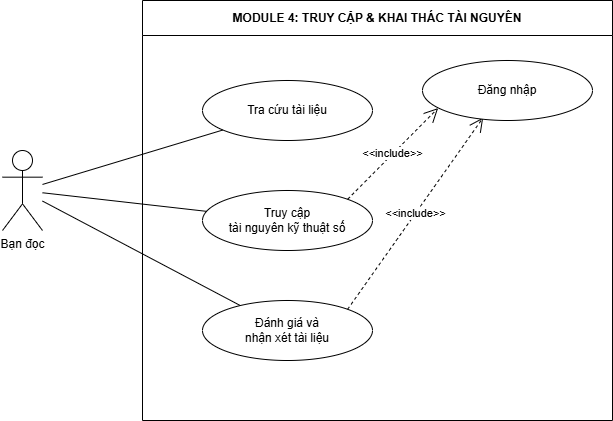
\includegraphics[width=0.8\linewidth]{Images/Truy_cap_khai_thac_tai_nguyen.png}
    \vspace{10pt}
    \caption{Sơ đồ Use-case Truy cập \& khai thác tài nguyên}
    \label{fig:usecase_exploration}
\end{figure}

\subsubsection{Đặc tả chi tiết}

% --- UC: TRA CỨU TÀI LIỆU ---
\begin{longtable}{|p{3.5cm}|p{11.5cm}|}
    \hline
    \textbf{Tên Use-case} & \textbf{Tra cứu tài liệu} \\
    \hline
    \textbf{Use-case ID} & UC-EXP-01 \\
    \hline
    \textbf{Tổng quan} & Cho phép bạn đọc tìm kiếm các tài liệu có trong thư viện thông qua các từ khóa cơ bản như Nhan đề, Tác giả, Thể loại hoặc mã ISBN. \\
    \hline
    \textbf{Actor} & Bạn đọc (Bao gồm cả khách chưa đăng nhập) \\
    \hline
    \textbf{Tiền điều kiện} & Hệ thống đang hoạt động và có kết nối cơ sở dữ liệu. \\
    \hline
    \textbf{Điều kiện kích hoạt} & Bạn đọc nhập từ khóa vào thanh tìm kiếm và nhấn "Tìm kiếm" (hoặc Enter). \\
    \hline
    \textbf{Các bước} & 
    1. Bạn đọc chọn tiêu chí tìm kiếm (Tất cả, Nhan đề, Tác giả...) và nhập từ khóa.\newline
    2. Hệ thống tiếp nhận từ khóa và truy vấn vào cơ sở dữ liệu danh mục.\newline
    3. Hệ thống trả về danh sách các kết quả phù hợp, phân trang (nếu nhiều kết quả).\newline
    4. Giao diện hiển thị các thông tin cơ bản của tài liệu: Ảnh bìa, Tên sách, Tác giả, Năm xuất bản và Trạng thái (Còn bản vật lý / Có bản Digital).\newline
    5. Bạn đọc nhấp vào một kết quả để xem trang chi tiết tài liệu. \\
    \hline
    \textbf{Hậu điều kiện} & Không làm thay đổi trạng thái của hệ thống. \\
    \hline
    \textbf{Xử lý ngoại lệ} & 
    Ex1: Không có tài liệu nào khớp với từ khóa $\rightarrow$ Hệ thống hiển thị thông báo "Không tìm thấy tài liệu phù hợp với từ khóa của bạn" và gợi ý các từ khóa khác hoặc kiểm tra lại chính tả. \\
    \hline
    \caption{Đặc tả Use-case Tra cứu tài liệu}
\end{longtable}

\newpage
% --- UC: TRUY CẬP TÀI NGUYÊN KỸ THUẬT SỐ ---
\begin{longtable}{|p{3.5cm}|p{11.5cm}|}
    \hline
    \textbf{Tên Use-case} & \textbf{Truy cập tài nguyên kỹ thuật số} \\
    \hline
    \textbf{Use-case ID} & UC-EXP-02 \\
    \hline
    \textbf{Tổng quan} & Bạn đọc xem trực tuyến (đọc E-book) các tài liệu số đã được thư viện tích hợp trên hệ thống. \\
    \hline
    \textbf{Actor} & Bạn đọc \\
    \hline
    \textbf{Tiền điều kiện} & Tài liệu đang xem có định dạng kỹ thuật số (PDF). \\
    \hline
    \textbf{Điều kiện kích hoạt} & Bạn đọc nhấn nút "Đọc trực tuyến" hoặc "Nghe sách nói" tại trang chi tiết tài liệu. \\
    \hline
    \textbf{Các bước} & 
    1. \textbf{[Include]} Hệ thống kiểm tra và yêu cầu thực hiện luồng "Đăng nhập" nếu bạn đọc chưa xác thực.\newline
    2. Hệ thống kiểm tra quyền truy cập của Bạn đọc đối với tài nguyên số này (có bị khóa tài khoản không).\newline
    3. Hệ thống kiểm tra giới hạn truy cập đồng thời (Ví dụ: Thư viện chỉ mua bản quyền cho 5 người đọc cùng lúc).\newline
    4. Nếu thỏa mãn, hệ thống mở trình xem tài liệu tích hợp (PDF Viewer) trên trình duyệt.\newline
    5. Hệ thống ghi nhận lịch sử truy cập tài liệu số của bạn đọc. \\
    \hline
    \textbf{Hậu điều kiện} & Phiên truy cập tài liệu số được thiết lập và ghi log. \\
    \hline
    \textbf{Xử lý ngoại lệ} & 
    Ex1: Vượt quá số lượng người dùng truy cập đồng thời $\rightarrow$ Hệ thống thông báo "Tất cả các bản sao kỹ thuật số hiện đang được sử dụng. Vui lòng thử lại sau". \\
    \hline
    \caption{Đặc tả Use-case Truy cập tài nguyên kỹ thuật số}
\end{longtable}

% --- UC: ĐÁNH GIÁ VÀ NHẬN XÉT TÀI LIỆU ---
\begin{longtable}{|p{3.5cm}|p{11.5cm}|}
    \hline
    \textbf{Tên Use-case} & \textbf{Đánh giá và nhận xét tài liệu} \\
    \hline
    \textbf{Use-case ID} & UC-EXP-03 \\
    \hline
    \textbf{Tổng quan} & Cho phép bạn đọc để lại số sao đánh giá (từ 1 đến 5 sao) và viết nhận xét bằng văn bản cho một tài liệu nhằm chia sẻ cảm nhận với cộng đồng thư viện. \\
    \hline
    \textbf{Actor} & Bạn đọc \\
    \hline
    \textbf{Tiền điều kiện} & Bạn đọc phải từng mượn bản vật lý hoặc truy cập bản kỹ thuật số của tài liệu này (để tránh đánh giá ảo/spam). \\
    \hline
    \textbf{Điều kiện kích hoạt} & Bạn đọc cuộn xuống phần Đánh giá trong trang chi tiết sách và nhấn "Viết nhận xét". \\
    \hline
    \textbf{Các bước} & 
    1. \textbf{[Include]} Hệ thống kiểm tra và yêu cầu thực hiện luồng "Đăng nhập".\newline
    2. Hệ thống đối chiếu lịch sử mượn/đọc của Bạn đọc với tài liệu hiện tại.\newline
    3. Giao diện hiển thị biểu mẫu bao gồm bộ chọn số sao (1-5) và khung nhập văn bản (tùy chọn).\newline
    4. Bạn đọc chọn số sao, nhập nội dung (nếu muốn) và nhấn "Gửi đánh giá".\newline
    5. Hệ thống validate nội dung (kiểm tra từ ngữ phản cảm).\newline
    6. Hệ thống lưu đánh giá vào cơ sở dữ liệu, tính toán lại điểm đánh giá trung bình của tài liệu.\newline
    7. Thông báo "Cảm ơn bạn đã đánh giá" và cập nhật giao diện hiển thị. \\
    \hline
    \textbf{Hậu điều kiện} & Dữ liệu đánh giá được lưu. Điểm đánh giá trung bình của tài liệu (Average Rating) được cập nhật. \\
    \hline
    \textbf{Xử lý ngoại lệ} & 
    Ex1: Bạn đọc chưa từng mượn/đọc tài liệu $\rightarrow$ Hệ thống ẩn nút hoặc hiện thông báo "Bạn cần mượn hoặc đọc tài liệu này trước khi có thể để lại nhận xét".\newline
    Ex2: Nhận xét chứa từ khóa vi phạm tiêu chuẩn cộng đồng $\rightarrow$ Hệ thống chặn lưu và thông báo "Nội dung nhận xét chứa từ ngữ không phù hợp". \\
    \hline
    \caption{Đặc tả Use-case Đánh giá và nhận xét tài liệu}
\end{longtable}


% ======================================================================================
% 4.5 TƯƠNG TÁC THÔNG MINH VÀ AI
% ======================================================================================
\subsection{Tương tác thông minh}

\subsubsection{Tổng quan}
\begin{figure}[H]
    \centering
    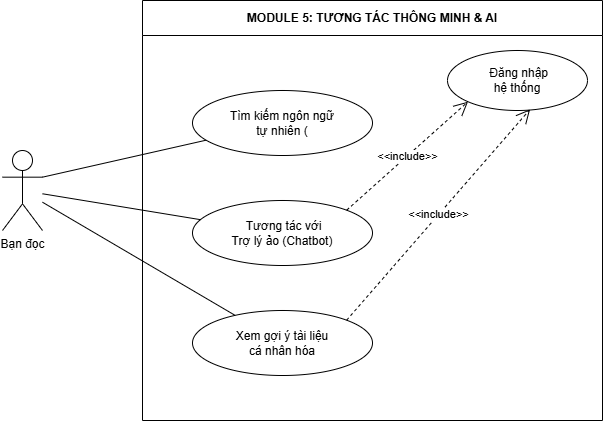
\includegraphics[width=0.8\linewidth]{Images/Tuong_tac_thong_minh_AI.png}
    \vspace{10pt}
    \caption{Sơ đồ Use-case Tương tác thông minh \& AI}
    \label{fig:usecase_smart_ai}
\end{figure}

\subsubsection{Đặc tả chi tiết}

% --- UC: TÌM KIẾM NGÔN NGỮ TỰ NHIÊN ---
\begin{longtable}{|p{3.5cm}|p{11.5cm}|}
    \hline
    \textbf{Tên Use-case} & \textbf{Tìm kiếm ngôn ngữ tự nhiên } \\
    \hline
    \textbf{Use-case ID} & UC-AI-01 \\
    \hline
    \textbf{Tổng quan} & Cho phép bạn đọc tra cứu tài liệu bằng cách gõ các câu truy vấn tự nhiên (VD: "sách về trí tuệ nhân tạo cơ bản") thay vì chỉ nhập từ khóa chính xác. \\
    \hline
    \textbf{Actor} & Bạn đọc  \\
    \hline
    \textbf{Tiền điều kiện} & Mô-đun AI NLP (Xử lý ngôn ngữ tự nhiên) của hệ thống đang hoạt động bình thường. \\
    \hline
    \textbf{Điều kiện kích hoạt} & Bạn đọc nhập câu truy vấn vào thanh tìm kiếm thông minh và nhấn "Tìm kiếm". \\
    \hline
    \textbf{Các bước} & 
    1. Bạn đọc nhập một câu văn hoặc cụm từ mô tả nhu cầu tìm sách.\newline
    2. Mô-đun AI tiếp nhận truy vấn và tiến hành Phân tích ý định (Intent Analysis) \& Trích xuất thực thể (Entity Extraction) để lấy ra các trường thông tin (Thể loại, chủ đề, đối tượng độc giả).\newline
    3. Hệ thống chuyển đổi các thực thể này thành biểu diễn vector (Vector Embeddings) hoặc truy vấn siêu dữ liệu phức hợp.\newline
    4. Tìm kiếm trong cơ sở dữ liệu và đánh giá mức độ tương đồng ngữ nghĩa (Semantic Ranking).\newline
    5. Hệ thống trả về danh sách các tài liệu liên quan nhất, sắp xếp theo điểm phù hợp từ cao xuống thấp. \\
    \hline
    \textbf{Hậu điều kiện} & Kết quả tìm kiếm được hiển thị kèm các gợi ý từ khóa liên quan. \\
    \hline
    \textbf{Xử lý ngoại lệ} & 
    Ex1: Câu truy vấn vô nghĩa hoặc không có kết quả phù hợp $\rightarrow$ Trợ lý AI phản hồi "Xin lỗi, tôi không tìm thấy tài liệu phù hợp với mô tả của bạn. Bạn có thể thử các cụm từ khác như...".\newline
    Ex2: Mô-đun AI bị lỗi hoặc quá tải $\rightarrow$ Hệ thống tự động chuyển (Fallback) về chế độ tìm kiếm từ khóa cơ bản (Full-text search) và thông báo "Tính năng tìm kiếm thông minh đang bảo trì". \\
    \hline
    \caption{Đặc tả Use-case Tìm kiếm ngôn ngữ tự nhiên}
\end{longtable}

\newpage
% --- UC: TƯƠNG TÁC VỚI TRỢ LÝ ẢO (CHATBOT) ---
\begin{longtable}{|p{3.5cm}|p{11.5cm}|}
    \hline
    \textbf{Tên Use-case} & \textbf{Tương tác với Trợ lý ảo (Chatbot)} \\
    \hline
    \textbf{Use-case ID} & UC-AI-02 \\
    \hline
    \textbf{Tổng quan} & Bạn đọc giao tiếp với Chatbot tích hợp AI để được giải đáp các quy định, nội quy thư viện, hoặc hỗ trợ tra cứu tình trạng mượn trả của cá nhân. \\
    \hline
    \textbf{Actor} & Bạn đọc \\
    \hline
    \textbf{Tiền điều kiện} & Dịch vụ Chatbot (AI Engine) đang trực tuyến. \\
    \hline
    \textbf{Điều kiện kích hoạt} & Bạn đọc mở cửa sổ Chatbot ở góc màn hình. \\
    \hline
    \textbf{Các bước} & 
    1. \textbf{[Include]} Hệ thống kiểm tra, nếu Bạn đọc chưa đăng nhập, Chatbot sẽ yêu cầu "Vui lòng đăng nhập để tôi có thể hỗ trợ các thông tin cá nhân của bạn tốt nhất". (Kích hoạt luồng Đăng nhập).\newline
    2. Giao diện Chatbot hiển thị lời chào kèm các nút thao tác nhanh (FAQ, Kiểm tra sách mượn, Gợi ý sách).\newline
    3. Bạn đọc nhập tin nhắn hoặc chọn một nút thao tác.\newline
    4. Chatbot (LLM) phân tích ngữ cảnh câu hỏi.\newline
    - Nếu là câu hỏi chung (FAQ): Trích xuất kiến thức từ bộ RAG (Retrieval-Augmented Generation) của thư viện để trả lời.\newline
    - Nếu là câu hỏi cá nhân (VD: "Tôi đang nợ sách gì?"): Chatbot gọi API vào hệ thống, truy xuất dữ liệu từ ID của Bạn đọc và tạo câu trả lời tự nhiên.\newline
    5. Giao diện hiển thị câu trả lời của Chatbot cho Bạn đọc. \\
    \hline
    \textbf{Hậu điều kiện} & Lịch sử đoạn chat được hệ thống lưu lại để phân tích và cải thiện mô hình AI. \\
    \hline
    \textbf{Xử lý ngoại lệ} & 
    Ex1: Chatbot không hiểu câu hỏi hoặc câu hỏi nằm ngoài phạm vi thư viện $\rightarrow$ Trả lời "Xin lỗi, tôi chỉ là trợ lý ảo hỗ trợ các nghiệp vụ thư viện. Vui lòng liên hệ thủ thư qua số hotline để được giải đáp cụ thể." \\
    \hline
    \caption{Đặc tả Use-case Tương tác với Trợ lý ảo (Chatbot)}
\end{longtable}

\newpage
% --- UC: XEM GỢI Ý TÀI LIỆU CÁ NHÂN HÓA ---
\begin{longtable}{|p{3.5cm}|p{11.5cm}|}
    \hline
    \textbf{Tên Use-case} & \textbf{Xem gợi ý tài liệu cá nhân hóa} \\
    \hline
    \textbf{Use-case ID} & UC-AI-03 \\
    \hline
    \textbf{Tổng quan} & Cung cấp cho bạn đọc danh sách các tài liệu được đề xuất riêng dựa trên lịch sử hoạt động, sở thích và hành vi của người dùng có chung sở thích. \\
    \hline
    \textbf{Actor} & Bạn đọc \\
    \hline
    \textbf{Tiền điều kiện} & Mô-đun AI Recommendation đang hoạt động. \\
    \hline
    \textbf{Điều kiện kích hoạt} & Bạn đọc truy cập vào trang chủ (Dashboard) hoặc trang "Gợi ý cho bạn". \\
    \hline
    \textbf{Các bước} & 
    1. \textbf{[Include]} Bạn đọc phải thực hiện "Đăng nhập" để hệ thống định danh.\newline
    2. Hệ thống thu thập các tín hiệu từ tài khoản người dùng: Lịch sử mượn, từ khóa tìm kiếm gần đây, điểm đánh giá sách (Rating).\newline
    3. Hệ thống gửi dữ liệu đến Mô-đun AI.\newline
    4. Mô-đun AI áp dụng thuật toán Lọc cộng tác (Collaborative Filtering) và Lọc theo nội dung (Content-based) để tính toán danh sách sách phù hợp.\newline
    5. Hệ thống lọc bỏ các tài liệu Bạn đọc đang mượn hoặc đã đặt giữ chỗ.\newline
    6. Hiển thị danh sách kết quả lên mục "Dành riêng cho bạn", kèm theo lý do gợi ý ngắn gọn (VD: "Vì bạn đã đọc cuốn X..."). \\
    \hline
    \textbf{Hậu điều kiện} & Giao diện hiển thị danh sách sách gợi ý, nâng cao trải nghiệm người dùng. \\
    \hline
    \textbf{Xử lý ngoại lệ} & 
    Ex1: Bạn đọc mới tạo tài khoản, chưa có bất kỳ lịch sử giao dịch nào (Cold Start Problem) $\rightarrow$ Hệ thống chuyển sang hiển thị danh sách "Các tài liệu phổ biến nhất" hoặc "Tài liệu mới nổi bật". \\
    \hline
    \caption{Đặc tả Use-case Xem gợi ý tài liệu cá nhân hóa}
\end{longtable}


% ======================================================================================
% 4.6 THÔNG BÁO VÀ TRUYỀN THÔNG
% ======================================================================================
\subsection{Thông báo và truyền thông}

\subsubsection{Tổng quan}
\begin{figure}[H]
    \centering
    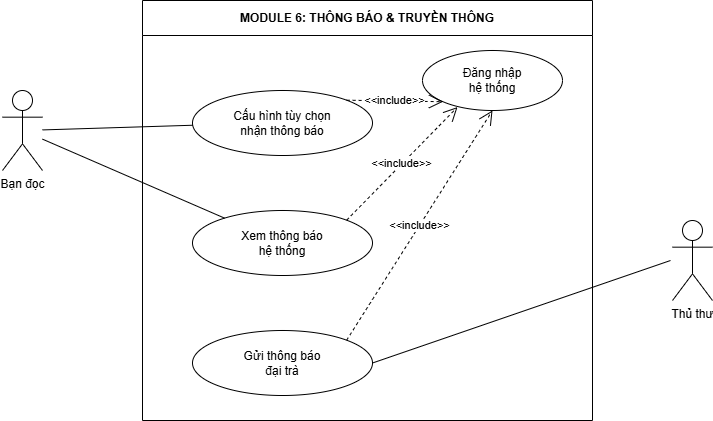
\includegraphics[width=0.8\linewidth]{Images/Thong_bao_truyen_thong.png}
    
    \vspace{10pt}
    \caption{Sơ đồ Use-case Thông báo \& truyền thông}
    \label{fig:usecase_notifications}
\end{figure}

\subsubsection{Đặc tả chi tiết}

% --- UC: CẤU HÌNH TÙY CHỌN NHẬN THÔNG BÁO ---
\begin{longtable}{|p{3.5cm}|p{11.5cm}|}
    \hline
    \textbf{Tên Use-case} & \textbf{Cấu hình tùy chọn nhận thông báo} \\
    \hline
    \textbf{Use-case ID} & UC-NOT-01 \\
    \hline
    \textbf{Tổng quan} & Cho phép bạn đọc tùy chỉnh các kênh nhận thông báo (Email, SMS, In-app) và loại thông báo muốn nhận (Nhắc trả sách, Sách đặt chỗ đã về, Thông báo hệ thống). \\
    \hline
    \textbf{Actor} & Bạn đọc \\
    \hline
    \textbf{Tiền điều kiện} & Bạn đọc có tài khoản hợp lệ trên hệ thống. \\
    \hline
    \textbf{Điều kiện kích hoạt} & Bạn đọc truy cập vào mục "Cài đặt thông báo" trong trang Hồ sơ cá nhân. \\
    \hline
    \textbf{Các bước} & 
    1. \textbf{[Include]} Hệ thống yêu cầu Bạn đọc thực hiện luồng "Đăng nhập hệ thống".\newline
    2. Hệ thống truy xuất và hiển thị trạng thái cấu hình thông báo hiện tại của tài khoản.\newline
    3. Bạn đọc thực hiện bật/tắt (toggle) các tùy chọn kênh liên lạc (Email, SMS) và các sự kiện muốn nhận thông báo.\newline
    4. Bạn đọc nhấn nút "Lưu cài đặt".\newline
    5. Hệ thống kiểm tra và cập nhật các tùy chọn mới vào cơ sở dữ liệu.\newline
    6. Hiển thị thông báo "Cập nhật cấu hình thông báo thành công". \\
    \hline
    \textbf{Hậu điều kiện} & Hệ thống chỉ gửi thông báo theo đúng các tùy chọn mà người dùng đã thiết lập. \\
    \hline
    \textbf{Xử lý ngoại lệ} & 
    Ex1: Bạn đọc chọn nhận thông báo qua SMS nhưng chưa cập nhật số điện thoại trong hồ sơ $\rightarrow$ Hệ thống cảnh báo "Vui lòng cập nhật số điện thoại trước khi kích hoạt tính năng này" và chuyển hướng đến trang cập nhật hồ sơ. \\
    \hline
    \caption{Đặc tả Use-case Cấu hình tùy chọn nhận thông báo}
\end{longtable}

\newpage
% --- UC: XEM THÔNG BÁO HỆ THỐNG ---
\begin{longtable}{|p{3.5cm}|p{11.5cm}|}
    \hline
    \textbf{Tên Use-case} & \textbf{Xem thông báo hệ thống} \\
    \hline
    \textbf{Use-case ID} & UC-NOT-02 \\
    \hline
    \textbf{Tổng quan} & Người dùng kiểm tra và đọc các cảnh báo, nhắc nhở (Ví dụ: sắp đến hạn trả sách, tài liệu giữ chỗ đã sẵn sàng) ngay trên giao diện ứng dụng web. \\
    \hline
    \textbf{Actor} & Bạn đọc \\
    \hline
    \textbf{Tiền điều kiện} & Hệ thống có thông báo mới được gửi đến tài khoản của người dùng. \\
    \hline
    \textbf{Điều kiện kích hoạt} & Người dùng nhấn vào biểu tượng "Cái chuông" (Trung tâm thông báo) trên thanh điều hướng. \\
    \hline
    \textbf{Các bước} & 
    1. \textbf{[Include]} Hệ thống yêu cầu người dùng "Đăng nhập hệ thống" để định danh.\newline
    2. Hệ thống truy vấn cơ sở dữ liệu để lấy danh sách các thông báo theo ID của người dùng, sắp xếp theo thời gian mới nhất.\newline
    3. Giao diện hiển thị danh sách thông báo (phân biệt rõ trạng thái "Đã đọc" và "Chưa đọc").\newline
    4. Người dùng click vào một thông báo cụ thể để xem chi tiết.\newline
    5. Hệ thống cập nhật trạng thái của thông báo đó thành "Đã đọc" và giảm số lượng huy hiệu (badge đếm số) trên biểu tượng chuông. \\
    \hline
    \textbf{Hậu điều kiện} & Trạng thái thông báo chuyển sang "Đã đọc". \\
    \hline
    \textbf{Xử lý ngoại lệ} & 
    Ex1: Không có thông báo nào $\rightarrow$ Hiển thị màn hình trống với thông điệp "Bạn không có thông báo nào mới". \\
    \hline
    \caption{Đặc tả Use-case Xem thông báo hệ thống}
\end{longtable}

% --- UC: GỬI THÔNG BÁO ĐẠI TRÀ ---
\begin{longtable}{|p{3.5cm}|p{11.5cm}|}
    \hline
    \textbf{Tên Use-case} & \textbf{Gửi thông báo đại trà} \\
    \hline
    \textbf{Use-case ID} & UC-NOT-03 \\
    \hline
    \textbf{Tổng quan} & Cho phép Thủ thư tạo và gửi các thông báo mang tính chất thông tin chung (như lịch nghỉ lễ, đóng cửa bảo trì, quy định mới) đến toàn bộ hoặc một nhóm bạn đọc cụ thể. \\
    \hline
    \textbf{Actor} & Thủ thư \\
    \hline
    \textbf{Tiền điều kiện} & Tài khoản Thủ thư đang ở trạng thái hoạt động và được cấp quyền gửi thông báo. \\
    \hline
    \textbf{Điều kiện kích hoạt} & Thủ thư truy cập công cụ "Quản lý truyền thông/Gửi thông báo" trên trang quản trị. \\
    \hline
    \textbf{Các bước} & 
    1. \textbf{[Include]} Thủ thư phải thực hiện "Đăng nhập hệ thống" để xác thực quyền hạn.\newline
    2. Hệ thống hiển thị biểu mẫu tạo thông báo mới.\newline
    3. Thủ thư nhập các thông tin: Tiêu đề, Nội dung chi tiết, Kênh gửi (In-app, Email) và Nhóm đối tượng nhận (Tất cả, Sinh viên, Giảng viên).\newline
    4. Thủ thư nhấn nút "Gửi thông báo".\newline
    5. Hệ thống xác nhận lại yêu cầu để tránh gửi nhầm.\newline
    6. Hệ thống đưa thông báo vào hàng đợi (Message Queue) và tiến hành phát tán đến nhóm đối tượng đã chọn.\newline
    7. Hệ thống hiển thị thông báo "Gửi thành công" và ghi log hành động. \\
    \hline
    \textbf{Hậu điều kiện} & Thông báo được lưu vào cơ sở dữ liệu và chuyển đến trung tâm thông báo/email của nhóm người dùng đích. \\
    \hline
    \textbf{Xử lý ngoại lệ} & 
    Ex1: Tiêu đề hoặc nội dung thông báo bị bỏ trống $\rightarrow$ Hệ thống vô hiệu hóa nút Gửi và cảnh báo "Vui lòng nhập đầy đủ nội dung thông báo". \\
    \hline
    \caption{Đặc tả Use-case Gửi thông báo đại trà}
\end{longtable}


% ======================================================================================
% 4.7 BÁO CÁO VÀ QUẢN TRỊ
% ======================================================================================
\subsection{Báo cáo và quản trị (Admin \& Reporting)}

\subsubsection{Tổng quan}
\begin{figure}[H]
    \centering
    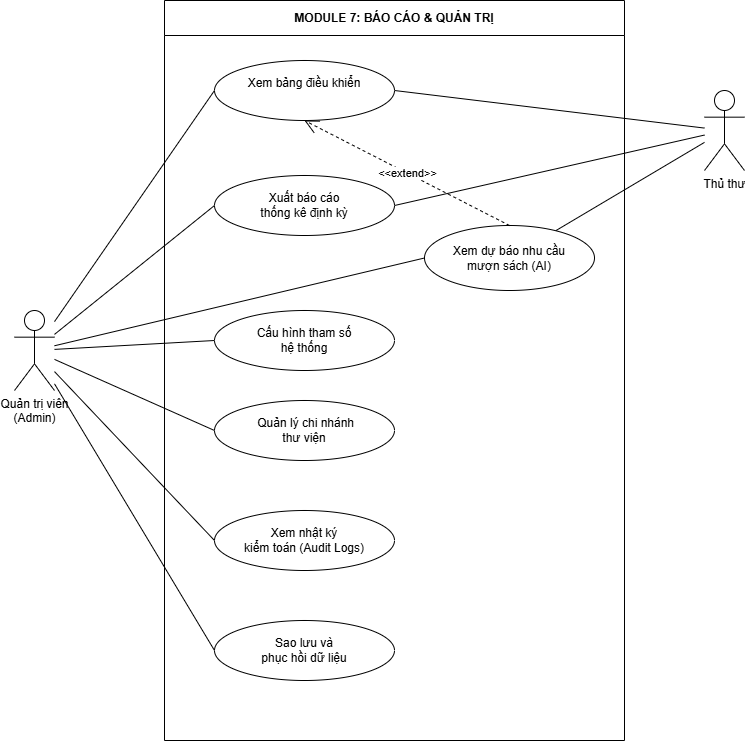
\includegraphics[width=0.8\linewidth]{Images/Bao_cao_quan_tri.png}
    \vspace{10pt}
    \caption{Sơ đồ Use-case Báo cáo \& Quản trị}
    \label{fig:usecase_admin}
\end{figure}

\subsubsection{Đặc tả chi tiết}

% --- UC: XEM BẢNG ĐIỀU KHIỂN ---
\begin{longtable}{|p{3.5cm}|p{11.5cm}|}
    \hline
    \textbf{Tên Use-case} & \textbf{Xem bảng điều khiển (Dashboard)} \\
    \hline
    \textbf{Use-case ID} & UC-ADM-01 \\
    \hline
    \textbf{Tổng quan} & Cung cấp giao diện tổng quan (thời gian thực) về các chỉ số hoạt động chính của thư viện như số sách đang mượn, sách quá hạn, lượt truy cập. \\
    \hline
    \textbf{Actor} & Quản trị viên (Admin), Thủ thư \\
    \hline
    \textbf{Tiền điều kiện} & Người dùng đã đăng nhập với vai trò Admin hoặc Thủ thư. \\
    \hline
    \textbf{Điều kiện kích hoạt} & Người dùng truy cập vào trang chủ của phân hệ quản trị. \\
    \hline
    \textbf{Các bước} & 
    1. Hệ thống tiếp nhận yêu cầu truy cập.\newline
    2. Truy vấn cơ sở dữ liệu để tổng hợp các số liệu thống kê trong ngày/tuần/tháng.\newline
    3. Trình bày dữ liệu dưới dạng các biểu đồ và thẻ thông tin (Cards).\newline
    \textit{** Điểm mở rộng (Extension Point):**}\newline
    - \textbf{[Extend]} Tại màn hình này, Thủ thư có thể kích hoạt tính năng \textit{"Xem dự báo nhu cầu mượn sách (AI)"} (UC-ADM-03) để xem các phân tích nâng cao. \\
    \hline
    \textbf{Hậu điều kiện} & Không làm thay đổi trạng thái dữ liệu của hệ thống. \\
    \hline
    \textbf{Xử lý ngoại lệ} & 
    Ex1: Hệ thống đang quá tải, không thể tải dữ liệu biểu đồ $\rightarrow$ Hiển thị thông báo "Dữ liệu đang được cập nhật, vui lòng thử lại sau" và hiển thị các số liệu cache gần nhất. \\
    \hline
    \caption{Đặc tả Use-case Xem bảng điều khiển}
\end{longtable}

\newpage
% --- UC: XUẤT BÁO CÁO THỐNG KÊ ĐỊNH KỲ ---
\begin{longtable}{|p{3.5cm}|p{11.5cm}|}
    \hline
    \textbf{Tên Use-case} & \textbf{Xuất báo cáo thống kê định kỳ} \\
    \hline
    \textbf{Use-case ID} & UC-ADM-02 \\
    \hline
    \textbf{Tổng quan} & Hỗ trợ trích xuất dữ liệu hoạt động của thư viện ra các định dạng tệp chuẩn (PDF, CSV, Excel) để phục vụ công tác lưu trữ và báo cáo cấp trên. \\
    \hline
    \textbf{Actor} & Quản trị viên (Admin), Thủ thư \\
    \hline
    \textbf{Tiền điều kiện} & Người dùng đã đăng nhập với vai trò hợp lệ. \\
    \hline
    \textbf{Điều kiện kích hoạt} & Người dùng chọn mục "Báo cáo thống kê" và nhấn "Xuất dữ liệu". \\
    \hline
    \textbf{Các bước} & 
    1. Hệ thống hiển thị biểu mẫu tùy chọn xuất báo cáo.\newline
    2. Người dùng chọn loại báo cáo (Tài liệu mượn nhiều nhất, Thu tiền phạt, Sách quá hạn), chọn mốc thời gian và định dạng tệp.\newline
    3. Người dùng nhấn nút "Xuất báo cáo".\newline
    4. Hệ thống thu thập dữ liệu, tiến hành định dạng và tạo tệp tin.\newline
    5. Hệ thống tự động tải tệp tin xuống thiết bị của người dùng. \\
    \hline
    \textbf{Hậu điều kiện} & Tệp báo cáo được tạo và tải về máy khách thành công. \\
    \hline
    \textbf{Xử lý ngoại lệ} & 
    Ex1: Không có dữ liệu trong khoảng thời gian đã chọn $\rightarrow$ Cảnh báo "Không có dữ liệu để xuất báo cáo". \\
    \hline
    \caption{Đặc tả Use-case Xuất báo cáo thống kê định kỳ}
\end{longtable}



% --- UC: CẤU HÌNH THAM SỐ HỆ THỐNG ---
\begin{longtable}{|p{3.5cm}|p{11.5cm}|}
    \hline
    \textbf{Tên Use-case} & \textbf{Cấu hình tham số hệ thống} \\
    \hline
    \textbf{Use-case ID} & UC-ADM-04 \\
    \hline
    \textbf{Tổng quan} & Thiết lập các quy tắc cốt lõi của thư viện như: Giới hạn số sách được mượn, thời hạn mượn, mức phạt trả trễ theo từng loại tài liệu. \\
    \hline
    \textbf{Actor} & Quản trị viên (Admin) \\
    \hline
    \textbf{Tiền điều kiện} & Admin đã đăng nhập vào hệ thống. \\
    \hline
    \textbf{Điều kiện kích hoạt} & Admin truy cập mục "Cài đặt hệ thống". \\
    \hline
    \textbf{Các bước} & 
    1. Hệ thống hiển thị các tham số cấu hình hiện tại.\newline
    2. Admin thay đổi các giá trị (Ví dụ: Tăng mức phạt trễ hạn từ 2000đ lên 5000đ/ngày).\newline
    3. Admin nhấn "Lưu cấu hình".\newline
    4. Hệ thống kiểm tra tính hợp lệ (không chứa giá trị âm, chuỗi ký tự sai).\newline
    5. Cập nhật vào cơ sở dữ liệu và ghi lại hành động vào Nhật ký kiểm toán. \\
    \hline
    \textbf{Hậu điều kiện} & Toàn bộ các luồng tính toán (phạt, hạn mượn) của hệ thống sẽ áp dụng theo tham số mới. \\
    \hline
    \textbf{Xử lý ngoại lệ} & 
    Ex1: Nhập giá trị không hợp lệ (nhập chữ vào ô số tiền) $\rightarrow$ Hệ thống báo lỗi và từ chối lưu. \\
    \hline
    \caption{Đặc tả Use-case Cấu hình tham số hệ thống}
\end{longtable}

% --- UC: QUẢN LÝ CHI NHÁNH THƯ VIỆN ---
\begin{longtable}{|p{3.5cm}|p{11.5cm}|}
    \hline
    \textbf{Tên Use-case} & \textbf{Quản lý chi nhánh thư viện} \\
    \hline
    \textbf{Use-case ID} & UC-ADM-05 \\
    \hline
    \textbf{Tổng quan} & Thêm, sửa, xóa thông tin các chi nhánh cơ sở trực thuộc, quản lý không gian vật lý của mạng lưới thư viện. \\
    \hline
    \textbf{Actor} & Quản trị viên (Admin) \\
    \hline
    \textbf{Tiền điều kiện} & Admin đã đăng nhập vào hệ thống. \\
    \hline
    \textbf{Điều kiện kích hoạt} & Admin truy cập menu "Quản lý chi nhánh". \\
    \hline
    \textbf{Các bước} & 
    1. Hệ thống hiển thị danh sách các chi nhánh hiện tại.\newline
    2. Admin chọn Thêm mới, Chỉnh sửa hoặc Xóa.\newline
    3. Admin điền thông tin chi nhánh (Tên, Địa chỉ, Số điện thoại, Quản lý chi nhánh).\newline
    4. Admin nhấn "Lưu".\newline
    5. Hệ thống cập nhật dữ liệu và hiển thị thông báo thành công. \\
    \hline
    \textbf{Hậu điều kiện} & Danh sách các chi nhánh được cập nhật. \\
    \hline
    \textbf{Xử lý ngoại lệ} & 
    Ex1: Xóa chi nhánh đang có dữ liệu sách hoặc nhân sự $\rightarrow$ Hệ thống từ chối xóa để bảo vệ toàn vẹn dữ liệu, yêu cầu thuyên chuyển tài sản/nhân sự trước khi xóa. \\
    \hline
    \caption{Đặc tả Use-case Quản lý chi nhánh thư viện}
\end{longtable}

\newpage
% --- UC: XEM NHẬT KÝ KIỂM TOÁN ---
\begin{longtable}{|p{3.5cm}|p{11.5cm}|}
    \hline
    \textbf{Tên Use-case} & \textbf{Xem nhật ký kiểm toán (Audit Logs)} \\
    \hline
    \textbf{Use-case ID} & UC-ADM-06 \\
    \hline
    \textbf{Tổng quan} & Tra cứu lịch sử các thao tác quan trọng đã được thực hiện trên hệ thống (ai làm gì, vào lúc nào) để phục vụ việc bảo mật và truy vết sự cố. \\
    \hline
    \textbf{Actor} & Quản trị viên (Admin) \\
    \hline
    \textbf{Tiền điều kiện} & Admin đã đăng nhập hệ thống. \\
    \hline
    \textbf{Điều kiện kích hoạt} & Admin truy cập mục "Nhật ký hệ thống". \\
    \hline
    \textbf{Các bước} & 
    1. Hệ thống truy xuất dữ liệu từ bảng Audit Log.\newline
    2. Hiển thị danh sách các sự kiện (Cập nhật cấu hình, Thêm tài khoản, Xóa sách...), sắp xếp theo thời gian mới nhất.\newline
    3. Admin có thể lọc dữ liệu theo Người thực hiện, khoảng thời gian hoặc mức độ rủi ro (Info, Warning, Critical).\newline
    4. Admin xem chi tiết dữ liệu trước và sau khi thay đổi (Old Data vs New Data). \\
    \hline
    \textbf{Hậu điều kiện} & Không làm thay đổi trạng thái của hệ thống. Dữ liệu này mang tính chất chỉ đọc (Read-only). \\
    \hline
    \textbf{Xử lý ngoại lệ} & Không có ngoại lệ đáng kể. \\
    \hline
    \caption{Đặc tả Use-case Xem nhật ký kiểm toán}
\end{longtable}

% --- UC: SAO LƯU VÀ PHỤC HỒI DỮ LIỆU ---
% \begin{longtable}{|p{3.5cm}|p{11.5cm}|}
%     \hline
%     \textbf{Tên Use-case} & \textbf{Sao lưu và phục hồi dữ liệu} \\
%     \hline
%     \textbf{Use-case ID} & UC-ADM-07 \\
%     \hline
%     \textbf{Tổng quan} & Đảm bảo an toàn dữ liệu hệ thống bằng cách sao lưu thủ công/tự động và khôi phục lại khi có sự cố. \\
%     \hline
%     \textbf{Actor} & Quản trị viên (Admin) \\
%     \hline
%     \textbf{Tiền điều kiện} & Admin đã đăng nhập với quyền hạn cao nhất. \\
%     \hline
%     \textbf{Điều kiện kích hoạt} & Admin truy cập mục "Quản trị dữ liệu". \\
%     \hline
%     \textbf{Các bước} & 
%     1. Màn hình hiển thị danh sách các bản sao lưu đã có và nút chức năng.\newline
%     2. Nếu chọn Sao lưu (Backup): Admin nhấn nút, hệ thống nén dữ liệu hiện tại và lưu trữ lên Server/Cloud.\newline
%     3. Nếu chọn Phục hồi (Restore): Admin chọn một bản sao lưu cũ, nhập mật khẩu cấp cao để xác nhận.\newline
%     4. Hệ thống tiến hành ghi đè dữ liệu hiện tại bằng dữ liệu từ bản sao lưu.\newline
%     5. Hệ thống khởi động lại dịch vụ và thông báo quá trình hoàn tất. \\
%     \hline
%     \textbf{Hậu điều kiện} & Dữ liệu được lưu trữ an toàn hoặc hệ thống được hoàn nguyên về trạng thái cũ. \\
%     \hline
%     \textbf{Xử lý ngoại lệ} & 
%     Ex1: Bản sao lưu bị hỏng (Corrupted) $\rightarrow$ Hệ thống cảnh báo lỗi khi cố gắng Restore và hủy bỏ tiến trình để bảo vệ dữ liệu hiện tại. \\
%     \hline
%     \caption{Đặc tả Use-case Sao lưu và phục hồi dữ liệu}
% \end{longtable}